\documentclass[11pt,a4paper]{report}%especifica o tipo de documento que tenciona escrever: carta, artigo, relatório... neste caso é um relatório
% [11pt,a4paper] Define o tamanho principal das letras do documento. caso não especifique uma delas, é assumido 10pt
% a4paper -- Define o tamanho do papel.
\usepackage{float}
\usepackage[portuges]{babel}%Babel -- irá activar automaticamente as regras apropriadas de hifenização para a língua todo o
                                   %-- o texto gerado é automaticamente traduzido para Português.
                                   %  Por exemplo, “chapter” irá passar a “capítulo”, “table of contents” a “conteúdo”.
                                   % portuges -- específica para o Português.
\usepackage[utf8]{inputenc} % define o encoding usado texto fonte (input)--usual "utf8" ou "latin1

\usepackage{graphicx} %permite incluir graficos, tabelas, figuras
\usepackage{url} % para utilizar o comando \url{}
\usepackage{enumerate} %permite escolher, nas listas enumeradas, se os iems sao marcados com letras ou numeros-romanos em vez de numeracao normal

%\usepackage{apalike} % gerar biliografia no estilo 'named' (apalike)

\usepackage{color} % Para escrever em cores

\usepackage{multirow} %tabelas com multilinhas
\usepackage{array} %formatação especial de tabelas em array

\usepackage[pdftex]{hyperref} % transformar as referências internas do seu documento em hiper-ligações.

%Exemplos de fontes -- nao e vulgar mudar o tipo de fonte
%\usepackage{tgbonum} % Fonte de letra: TEX Gyre Bonum
%\usepackage{lmodern} % Fonte de letra: Latin Modern Sans Serif
%\usepackage{helvet}  % Fonte de letra: Helvetica
%\usepackage{charter} % Fonte de letra:Charter

\definecolor{saddlebrown}{rgb}{0.55, 0.27, 0.07} % para definir uma nova cor, neste caso 'saddlebrown'

\usepackage{listings}  % para utilizar blocos de texto verbatim no estilo 'listings'
%paramerização mais vulgar dos blocos LISTING - GENERAL
\lstset{
	basicstyle=\small, %o tamanho das fontes que são usadas para o código
	numbers=left, % onde colocar a numeração da linha
	numberstyle=\tiny, %o tamanho das fontes que são usadas para a numeração da linha
	numbersep=5pt, %distancia entre a numeração da linha e o codigo
	breaklines=true, %define quebra automática de linha
    frame=tB,  % caixa a volta do codigo
	mathescape=true, %habilita o modo matemático
	escapeinside={(*@}{@*)} % se escrever isto  aceita tudo o que esta dentro das marcas e nao altera
}
%
%\lstset{ %
%	language=Java,							% choose the language of the code
%	basicstyle=\ttfamily\footnotesize,		% the size of the fonts that are used for the code
%	keywordstyle=\bfseries,					% set the keyword style
%	%numbers=left,							% where to put the line-numbers
%	numberstyle=\scriptsize,				% the size of the fonts that are used for the line-numbers
%	stepnumber=2,							% the step between two line-numbers. If it's 1 each line
%											% will be numbered
%	numbersep=5pt,							% how far the line-numbers are from the code
%	backgroundcolor=\color{white},			% choose the background color. You must add \usepackage{color}
%	showspaces=false,						% show spaces adding particular underscores
%	showstringspaces=false,					% underline spaces within strings
%	showtabs=false,							% show tabs within strings adding particular underscores
%	frame=none,								% adds a frame around the code
%	%abovecaptionskip=-.8em,
%	%belowcaptionskip=.7em,
%	tabsize=2,								% sets default tabsize to 2 spaces
%	captionpos=b,							% sets the caption-position to bottom
%	breaklines=true,						% sets automatic line breaking
%	breakatwhitespace=false,				% sets if automatic breaks should only happen at whitespace
%	title=\lstname,							% show the filename of files included with \lstinputlisting;
%											% also try caption instead of title
%	escapeinside={\%*}{*)},					% if you want to add a comment within your code
%	morekeywords={*,...}					% if you want to add more keywords to the set
%}

\usepackage{xspace} % deteta se a seguir a palavra tem uma palavra ou um sinal de pontuaçao se tiver uma palavra da espaço, se for um sinal de pontuaçao nao da espaço

\parindent=0pt %espaço a deixar para fazer a  indentação da primeira linha após um parágrafo
\parskip=2pt % espaço entre o parágrafo e o texto anterior

\setlength{\oddsidemargin}{-1cm} %espaço entre o texto e a margem
\setlength{\textwidth}{18cm} %Comprimento do texto na pagina
\setlength{\headsep}{-1cm} %espaço entre o texto e o cabeçalho
\setlength{\textheight}{23cm} %altura do texto na pagina

% comando '\def' usado para definir abreviatura (macros)
% o primeiro argumento é o nome do novo comando e o segundo entre chavetas é o texto original, ou sequência de controle, para que expande
\def\darius{\textsf{Darius}\xspace}
\def\antlr{\texttt{AnTLR}\xspace}
\def\pe{\emph{Publicação Eletrónica}\xspace}
\def\titulo#1{\section{#1}}    %no corpo do documento usa-se na forma '\titulo{MEU TITULO}'
\def\super#1{{\em Supervisor: #1}\\ }
\def\area#1{{\em \'{A}rea: #1}\\[0.2cm]}
\def\resumo{\underline{Resumo}:\\ }

%\input{LPgeneralDefintions} %permite ler de um ficheiro de texto externo mais definições

\title{Projeto de Arquiteturas de Software\\
       \textbf{Plataforma de Trading}\\ Relatório de Desenvolvimento
       } %Titulo do documento
%\title{Um Exemplo de Artigo em \LaTeX}
\author{José André Martins Pereira\\ (a82880@alunos.uminho.pt) \and Ricardo André Gomes Petronilho\\ (a81744@alunos.uminho.pt)
       } %autores do documento
\date{\today} %data

\begin{document} % corpo do documento
\maketitle % apresentar titulo, autor e data

\begin{abstract}  % resumo do documento
No Mestrado integrado de Engenharia Informática, na Unidade Curricular de Arquiteturas de Software foi-nos proposta a elaboração de um projeto de desenvolvimento de uma plataforma de trading.
\end{abstract}

\tableofcontents % Insere a tabela de indice
%\listoffigures % Insere a tabela de indice figuras
%\listoftables % Insere a tabela de indice tabelas

\chapter{Introdução} \label{chap:intro} %referência cruzada

No Mestrado integrado de Engenharia Informática, na unidade curricular de Arquiteturas de Software foi-nos proposta a elaboração de um projeto para o desenvolvimento de uma plataforma de trading.\\
A plataforma de trading tem como objetivo a realização de contratos de diferença (Contrats for Differences – CFD), podendo estes ser de venda ou compra de ativos.\\
Um \textbf{CFD de compra}, também designado \texrbf{CFD long} deverá ocorrer quando o utilizador tem a expectativa que o preço atual de um determinado ativo vai aumentar no futuro e  fechar o contrato, nessa mesma altura, para obter a diferença.\\
Um \textbf{CFD de venda}, também designado \textbf{CFD long} deverá ocorrer quando o utilizador tem a expectativa que o preço atual de um determinado ativo vai diminuir no futuro e  fechar o contrato, nessa mesma altura, para obter a diferença.\\
Ao longo deste relatório, especifica-se o processo de desenvolvimento da arquitetura para esta plataforma de trading.


\chapter{Desenvolvimento da Arquitetura}

\section{Funcionalidades}

\begin{itemize}
    \item Os traders/investidores podem criar uma conta com um plafond inicial para negociação/investimento.
    \item Os traders/investidores podem adicionar/remover fundos ao seu plafond.
    \item Os traders/investidores podem abrir posições (CFDs) sobre os ativos disponíveis, posições de venda e compra.
    \item Os traders/investidores podem encerrar um contrato por ação:\\
Direta – encerra a posição (CFDs) no momento.\\
Indireta - definir para as posições de venda e compra abertas limites de perda e ganho - Take profit (TP) e Stop Loss (SL) ).\\
    \item Os traders/investidores pode desativar o encerramento por ação indireta (remover os limites de SL ou TP).
    \item Os traders/investidores deverão poder monitorizar em ‘tempo real’ o seu portfolio atual (e de outros caso os mesmos consintam) de CFDs.

\end{itemize}{}

\section{Mockups}

\begin{figure}[H]
	\centering
	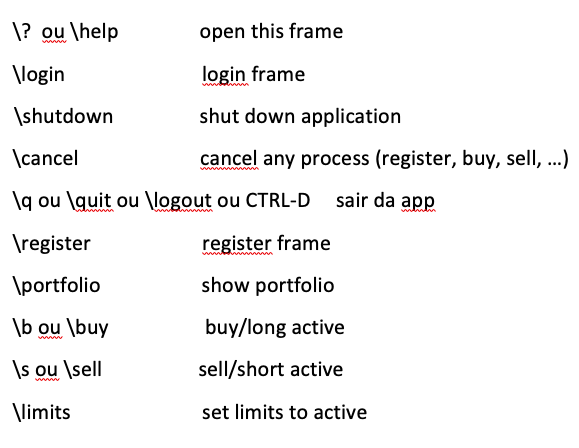
\includegraphics[scale=0.6]{ui1.png}
	\caption{escrever barra help lista todas as opções/funcionalidades da aplicação.}
	\label{img:pag}
\end{figure}

\begin{figure}[H]
	\centering
	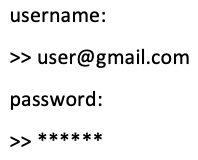
\includegraphics[scale=0.6]{ui2.png}
	\caption{Login do utilizador. }
	\label{img:pag}
\end{figure}

\begin{figure}[H]
	\centering
	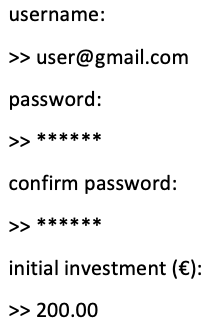
\includegraphics[scale=0.6]{ui3.png}
	\caption{Registo do utilizador. }
	\label{img:pag}
\end{figure}

\begin{figure}[H]
	\centering
	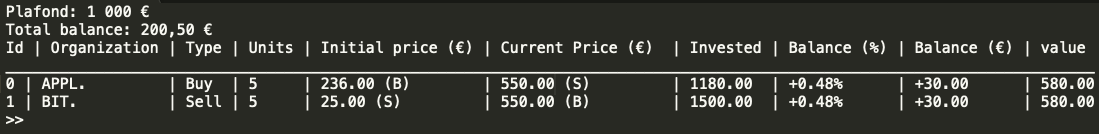
\includegraphics[scale=0.45]{ui4.png}
	\caption{Consultar portfolio. }
	\label{img:pag}
\end{figure}

\begin{figure}[H]
	\centering
	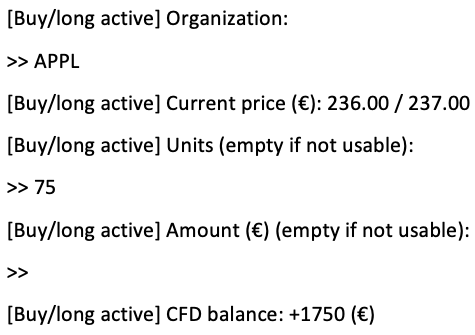
\includegraphics[scale=0.6]{ui5.png}
	\caption{Fazer um CFD de compra. }
	\label{img:pag}
\end{figure}

\begin{figure}[H]
	\centering
	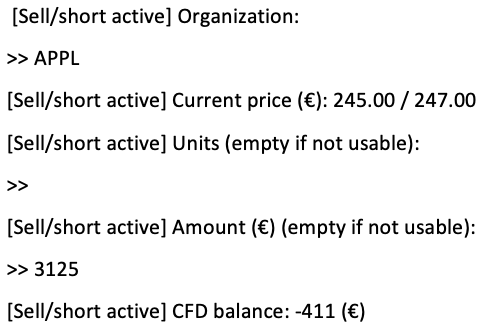
\includegraphics[scale=0.6]{ui6.png}
	\caption{Fazer um CFD de venda. }
	\label{img:pag}
\end{figure}

\begin{figure}[H]
	\centering
	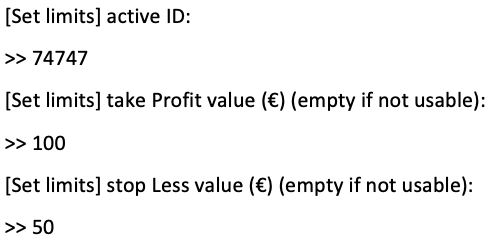
\includegraphics[scale=0.6]{ui7.png}
	\caption{Definir limites de stop less e take profit. }
	\label{img:pag}
\end{figure}

\newpage

\section{Modelo Domínio}

Devido às dimensões do modelo domínio, vamos apresentar o mesmo por partes. O primeiro subsistema que se vai abordar é o intitulado de recursos humanos, ou seja, responsável pelos utilizadores deste sistema. \\Todo o utilizador contém um username e password, pois são os dados comuns aos diferentes tipos, no entanto, achou-se importante distinguir dois tipos de utilizador do sistema, o administrador e trader, este último tem ainda associado um plafond, ou seja, o valor em carteira na aplicação. \\O trader pode assumir dois comportamentos no sistema, o de comprador e vendedor de ativos.\\
Por fim, e não menos importante, o utilizador pode consultar a lista de ativos existentes e a respetiva informação (valor atual, designação, ...), bem como o seu portfolio, ou seja, o conjunto de contratos realizados pelo mesmo, sendo que a associação do portfolio aos CFDs não é visível na imagem abaixo.

\begin{figure}[H]
	\centering
	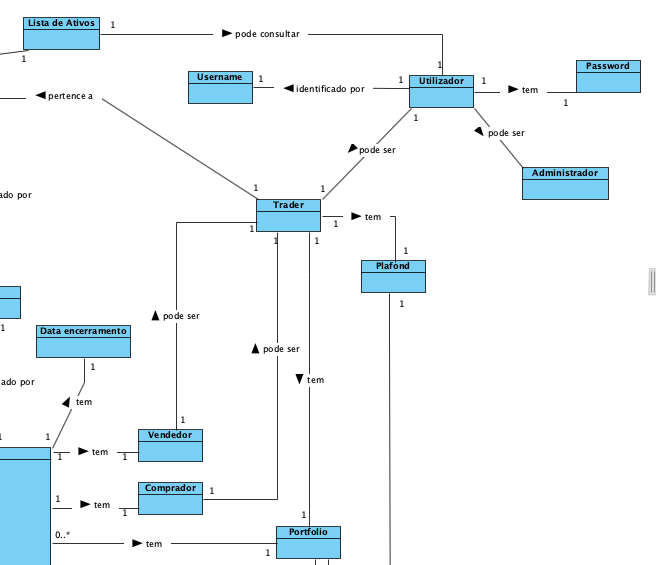
\includegraphics[scale=0.6]{modelo-dominio-1.png}
	\caption{Subsistema dos recursos humanos. }
	\label{img:pag}
\end{figure}

\newpage

O ativo tal como se pode verificar na figura abaixo, é identificado por um \textbf{id} (\emph{APPL.}), contém uma \textbf{designação}, normalmente associado à organização (\emph{APPLE}), dois tipos de valor, \textbf{valor de compra} e \textbf{venda}, e pode ser dividído em dois tipos:

\begin{itemize}
    \item Ação
    \item Commodities
\end{itemize}{}

O ativos do tipo \textbf{ação} está associado a uma organização enquanto que o \textbf{commodities} está a um recurso natural. Também é importante referir que vai existir uma \emph{Lista de ativos}, onde estão as informações de cada ativo.

\begin{figure}[H]
	\centering
	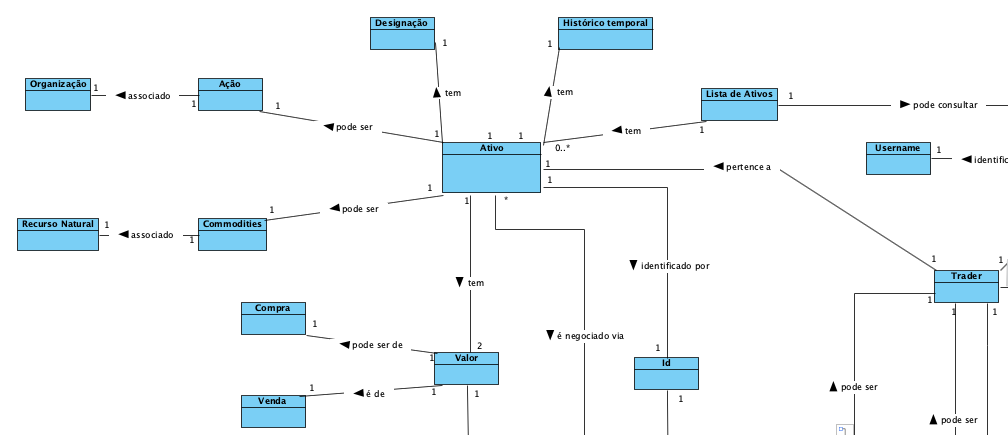
\includegraphics[scale=0.5]{modelo-dominio-2.png}
	\caption{Subsistema do ativo. }
	\label{img:pag}
\end{figure}
Tal como se pode verificar na figura abaixo, o CFD é um contrato de diferenças de uma determinada quantidade de ativos associado a uma organização ou recurso natural, sendo este identificado por um \textbf{id}. \\
Deste modo, existem dois tipos de \textbf{CFDs}, o \textbf{Long} e \textbf{Short}, que são respetivamente o \textbf{CFD de venda} e \textbf{compra}. \\Tal como o \textbf{ativo} o \textbf{CFD} também tem um valor de venda e compra, mas acresce ainda os campos de \textbf{valor investido} (total do valor dos ativos) e um \textbf{profit}, que são o agregado dos valores dos ativos.\\Existem duas formas de encerramento do \textbf{CFD}, por ação direta ou indireta. A ação direta, tal como o nome sugere, o encerramento é deliberado pelo utilizar no instante que a executar, a ação indireta é realizada através do estabelecimento de limites de \textbf{Stop less} e \textbf{Take profit}, tal como se pode verificar na figura abaixo.\\ Por fim, e não menos importante, através do ato de encerramento descrito anteriormente, o CFD tem dois estados possíveis, \textbf{aberto} e \textbf{encerrado}.

\begin{figure}[H]
	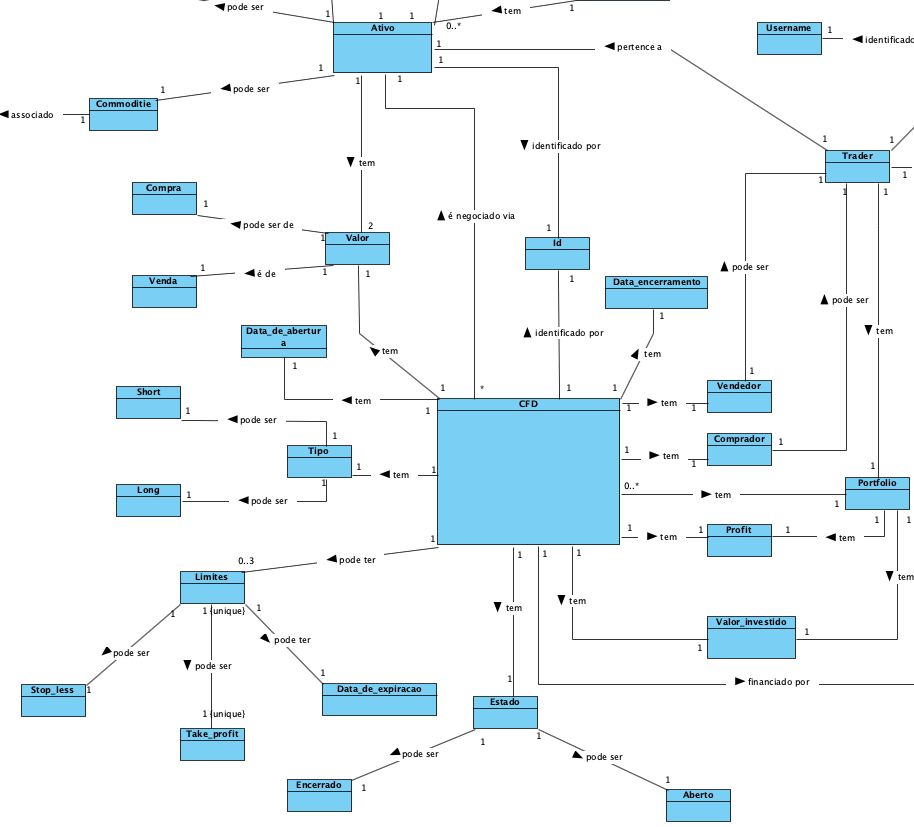
\includegraphics[scale=0.5]{modelo-dominio-3.png}
	\caption{Subsistema do CFD. }
	\label{img:pag}
\end{figure}

\newpage

\section{Diagrama de use cases}

Tal como se pode observar a figura abaixo, o diagrama de use cases é um reflexo das funcionalidades já listadas anteriormente, tendo este dois atores, o \textbf{trader} (cliente da aplicação) e o \textbf{administrador}. \\
Das funcionalidades presentes, as mais importantes em relação ao \textbf{cliente} são \textbf{Visualizar a lista de ativos}, que tal como o nome indica vai listar os ativos e a respetiva informação dos preços atuais de venda e compra e a organização a que estão associados, o \textbf{Abrir CFD}, responsável por começar um contrato. \\ No entanto, a funcionalidade mais importante de todo o sistema é o \textbf{Encerrar CFD}, sendo este responsável por calcular todos os valores finais do contrato. \\ Por fim, a funcionalidade mais importante do administrador é a \textbf{inicialização do trading system}, pois tal como já foi referenciado anteriormente, o sistema é capaz de executar encerramentos por ação indireta/automáticos através de limites. No entanto, isto só é garantido com um servidor que está \emph{full time} a verificar os \textbf{CFDs} que ultrapassam os limites de \textbf{Stop Less} e \textbf{Take Profit}. 

\begin{figure}[H]
	\centering
	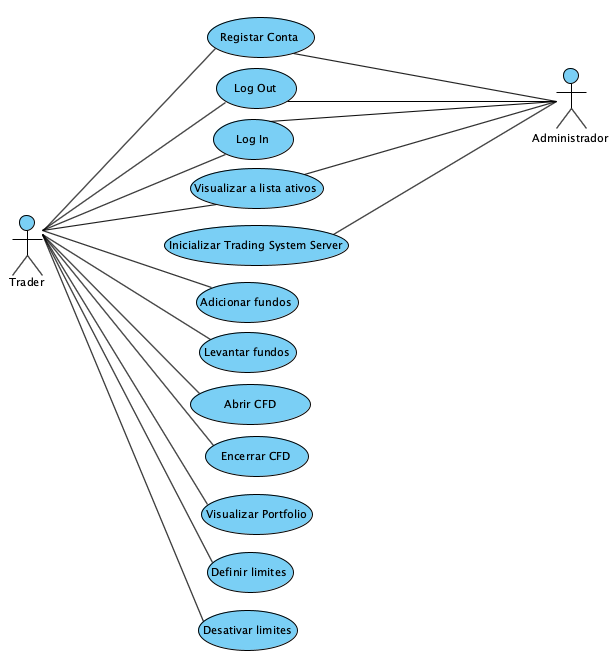
\includegraphics[scale=0.6]{diagrama-use-cases.png}
	\caption{Diagrama de use cases. }
	\label{img:pag}
\end{figure}

\newpage

\section{Atributos de qualidade}

O sistema ser \textbf{funcional} é o principal objetivo, no entanto são as \textbf{características não funcionais} ou \textbf{atributos de qualidade} que influenciam totalmente a conceção da solução arquitetural. Para a mesma funcionalidade podemos ter diferentes arquiteturas. Um sistema lento pode fornecer a mesma funcionaliade que outro mais rápido, neste caso o \textbf{desempenho} é o atributo de qualidade que influenciou as diferenças na solução.
\newline
\newline
A implementação interna da nossa aplicação, neste momento, realiza acessos a uma única base de dados, quando utilizada por vários utilizadores simultâneamente pode existir um pico de acessos à mesma.
\newline
Uma das soluções possíveis para resolver este declínio de desempenho é definir um limite temporal de \emph{queries} para cada utilizador.
\newline 
A seguinte figura ilustra um cenário em que um \textbf{Trader} consulta o seu porfolio para verificar os contratos (CFD's) em aberto.

\begin{figure}[H]
	\centering
	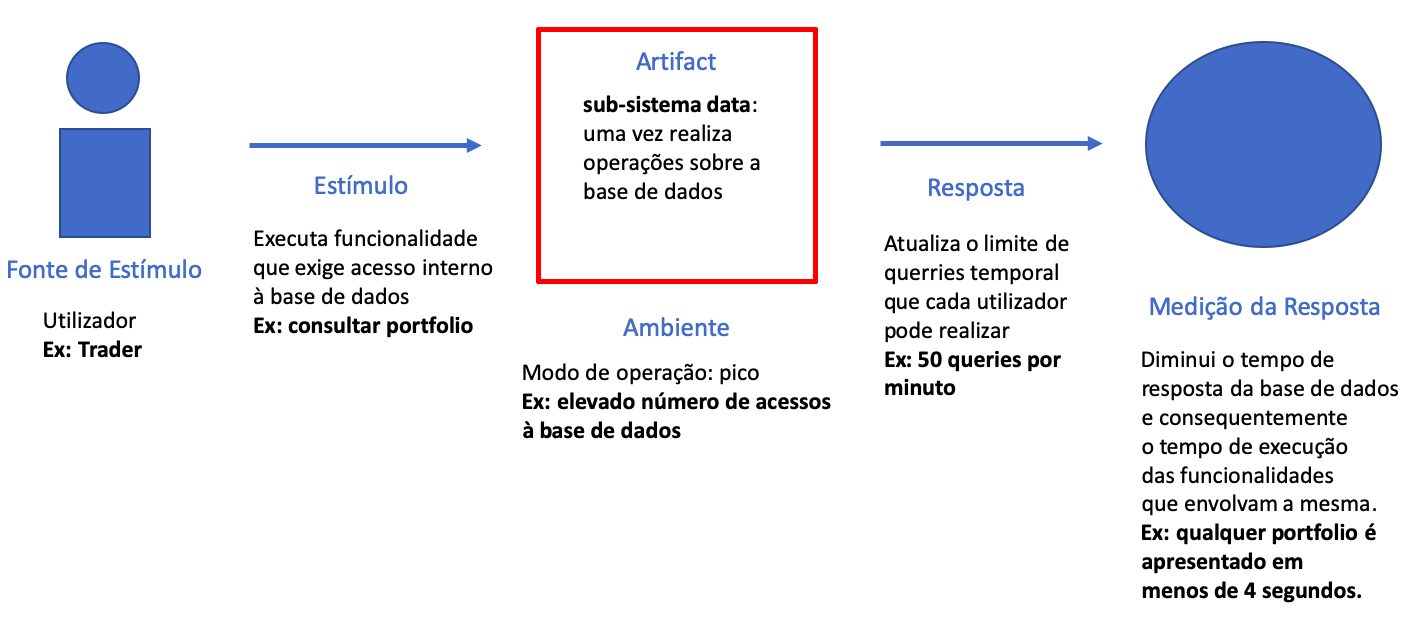
\includegraphics[scale=0.35]{AQ_performace.png}
	\caption{Cenário de performance. }
	\label{img:pag}
\end{figure}

\newpage

\section{Diagrama de classes}

O desenvolvimento do diagrama de classes foi baseado na arquitetura \emph{MVC}, sendo que dividiu-se o sistema em dois grandes \emph{packages}: \textbf{business} e \textbf{data}. \\No entanto, para reforçar a arquitetura, no \emph{package} \textbf{business}, foram criados dois  \emph{sub-packages}, pois a equipa achou clara a distinção entre o subsistema dos utilizadores, denominado por \textbf{recursos humanos} e o subsistema da lógica \textbf{trading}. Importante referir que para cada \emph{package} foi definida uma interface e uma classe \emph{Facade} que implementa a mesma com todos os métodos.\\
\newline
Em relação ao \emph{package} \textbf{data}, tal como se pode verificar na figura abaixo, caracteriaza-se pela comunicação com os dados, ou seja, a base de dados, bem como a \textbf{API} utilizada para obtenção dos valores reais dos ativos, nomeadamente a classe \textbf{AtivoDAO}. As restantes classes internas a este package são referentes aos \textbf{CFDs} e \textbf{Utilizadores}. Importante referir que os métodos presentes no \textbf{Facade} são nomeadamente inserção, remoção e listagem de dados.

\begin{figure}[H]
	\centering
	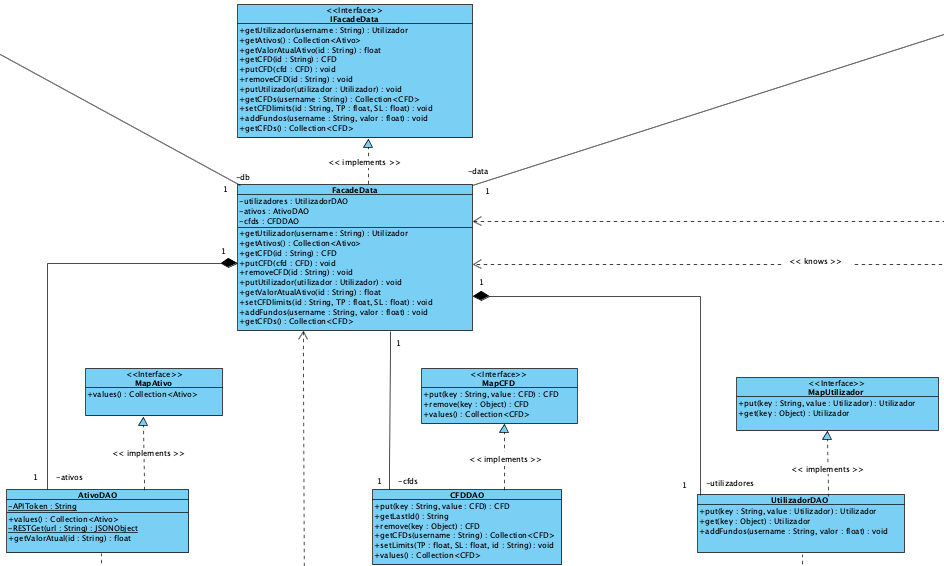
\includegraphics[scale=0.5]{diagrama-classes-1.png}
	\caption{Diagrama de classes, package data. }
	\label{img:pag}
\end{figure}

\newpage

A parte do diagrama de classes presente na figura abaixo, representa o \emph{package} \textbf{recursos humanos} denominado no diagrama por \textbf{RH}, que está inserido no \emph{package} \textbf{business}. Neste \emph{package} foi criado um \textbf{FacadeRH}, pois tal como já foi referido decidiu-se implementar uma classe \textbf{Facade} para cada \emph{package}. Nesta classe estão definidos os métodos de \textbf{registo}, \textbf{login} dos utilizadores, bem como a respetiva classe \textbf{Utilizador} e as suas sub-classes.

\begin{figure}[H]
	\centering
	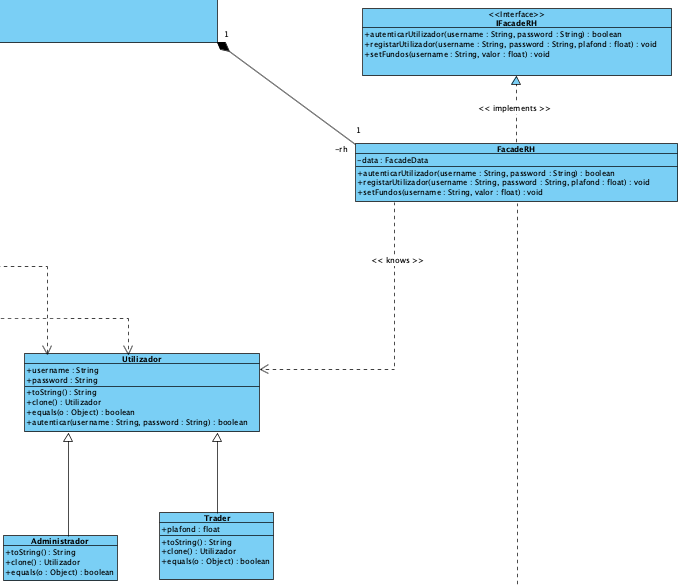
\includegraphics[scale=0.5]{diagrama-classes-2.png}
	\caption{Diagrama de classes, package business.RH. }
	\label{img:pag}
\end{figure}

Do mesmo modo, que o \emph{package} referido anteriormente, este incluí a interface \textbf{IFacadeTrading} e a classe \textbf{FacadeTrading}, onde estao definidos os métodos deste \emph{package}. O objetivo deste \emph{package} é concentrar as funcionalidades sobre os \textbf{CFDs} e os \textbf{Ativos}, tal como se pode verificar na figura abaixo. 

\begin{figure}[H]
	\centering
	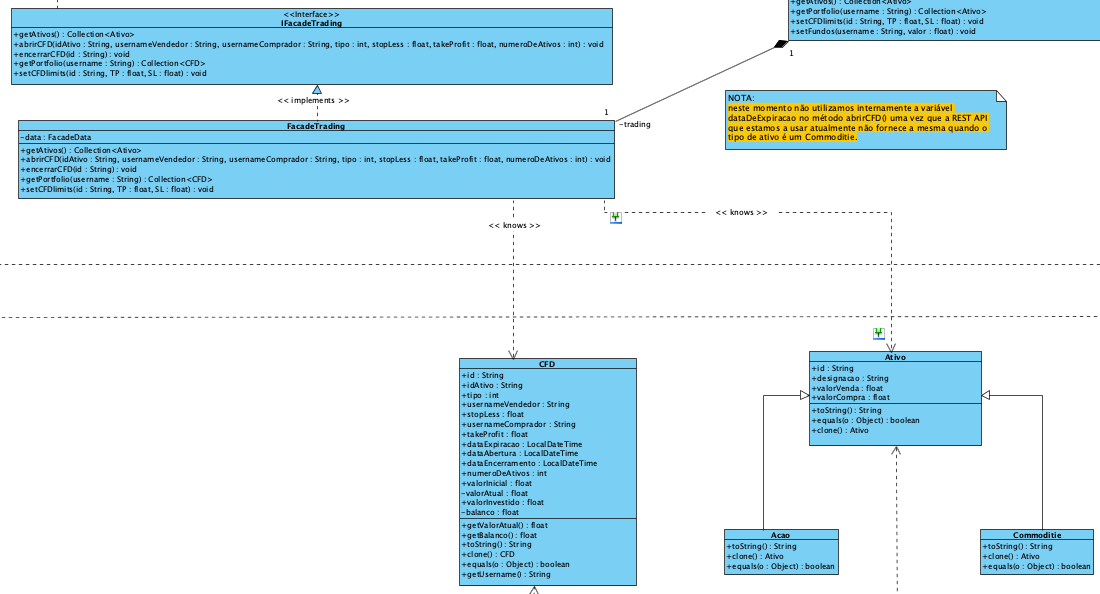
\includegraphics[scale=0.5]{diagrama-classes-3.png}
	\caption{Diagrama de classes, package business.Trading. }
	\label{img:pag}
\end{figure}

Tal como foi dito anteriormente e observando a figura abaixo, os \emph{packages} apresentados acima, estão inseridos no \emph{package} \textbf{business}. Igualmente aos anteriores, este \emph{package} também tem uma interface, denominada \textbf{IFacadeBusiness} e a classe \textbf{Facade} designada \textbf{FacadeBusiness}, onde estão implementados todos os métodos dos \emph{packages} \textbf{Trading} e \textbf{RH} e os atributos dos \textbf{Facades} dos mesmos (setas vermelhas), bem como o \textbf{FacadeData} para aceder aos dados.

\begin{figure}[H]
	\centering
	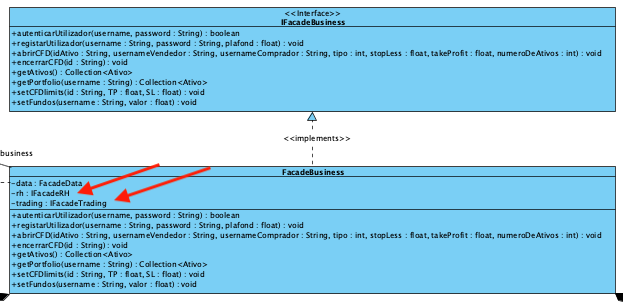
\includegraphics[scale=0.5]{diagrama-classes-4.png}
	\caption{Diagrama de classes, package business. }
	\label{img:pag}
\end{figure}

Tal como foi explicado inicialmente o utilizador pode encerrar um CFD automáticamente, definindo limites de \textbf{Top Less} e \textbf{Take profit}, o que significa que, a qualquer momento isso pode acontecer, mesmo quando o cliente não estiver autenticado na aplicação. Então a equipa decidiu que era necessário um servidor, para verificar os encerramentos automáticos dos \textbf{CFDs}, sendo este implementado na classe \textbf{TSServer}.

\begin{figure}[H]
	\centering
	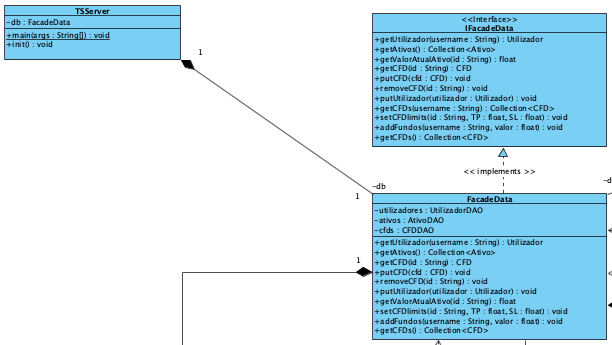
\includegraphics[scale=0.5]{diagrama-classes-5.png}
	\caption{Diagrama de classes, classe TSServer. }
	\label{img:pag}
\end{figure}

Por fim, a classe cental da arquitetura denominada por \textbf{TSClient}, onde estará desenvolvida a view do programa, bem como todas as funcionalidades do mesmo. Os atributos desta classe, são os \textbf{Facades} dos \emph{packages}.

\begin{figure}[H]
	\centering
	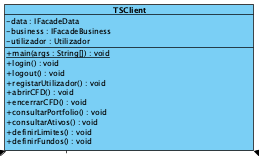
\includegraphics[scale=0.5]{diagrama-classes-6.png}
	\caption{Diagrama de classes, TSClient. }
	\label{img:pag}
\end{figure}

\newpage

\section{Diagramas de comportamento}

Nesta fase implementou-se o diagrama de sequência de implementação para a funcionalidade automática do sistema que consiste em verificar os contratos abertos (CFD's) de cada utilizador e caso os limites de Stop Less ou Take Profit sejam alcançados, é feito o encerramento do contrato (CFD).

\begin{figure}[H]
	\centering
	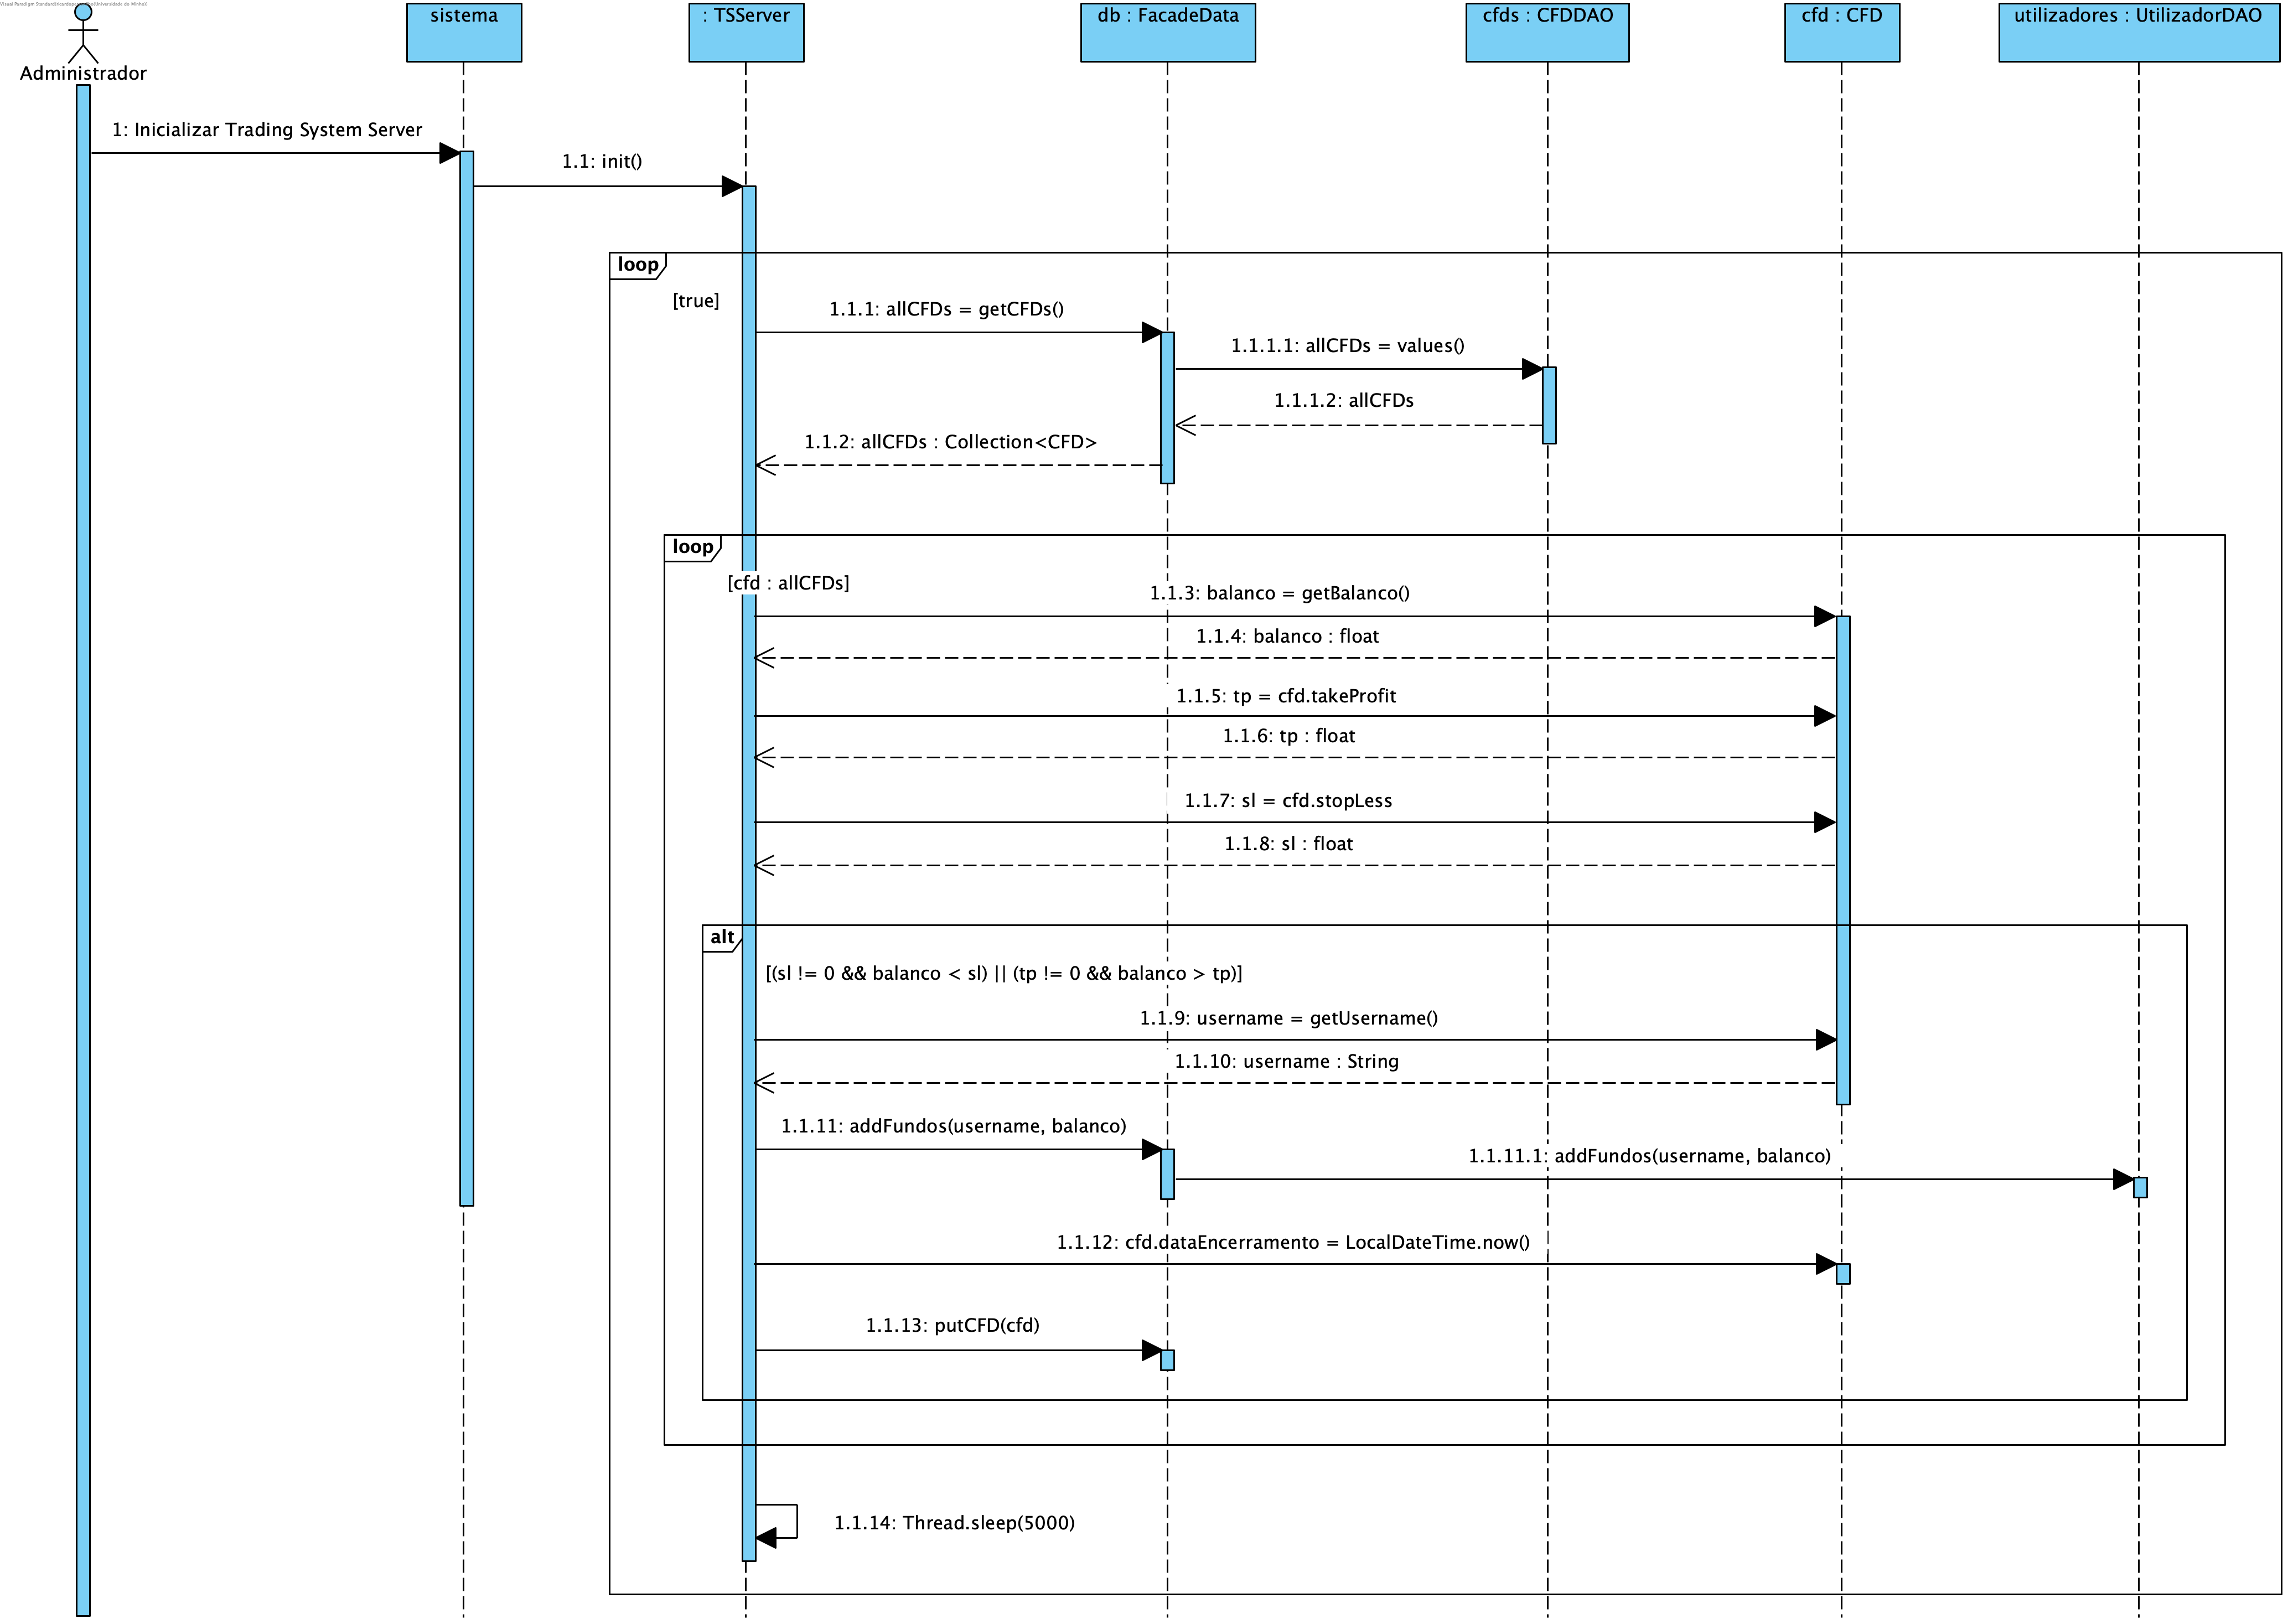
\includegraphics[scale=0.5]{Inicializar_Trading_System_Server.png}
	\caption{Diagrama de sequência de implementação. }
	\label{img:pag}
\end{figure}

No diagrama estão já especificadas as classes e variáveis envolventes tornando o futuro processo de implementação do método bastante facilitado uma vez que o raciocínio e fluxo de execução (comportamento) da funcionalidade está detalhada.

Note-se que a última execução do loop exterior é o método \textbf{Thread.sleep(5000)} uma vez que esta funcionalidade automática é realizada de 5 em 5 segundos, o intervalo pode ser ajustado conforme os resultados pertendidos.  


\newpage

\chapter{Conclusão}

Ao realizar esta fase do projeto a equipa apercebeu-se da importância de seguir o processo de desenvolvimento de software pela ordem indicada pelos professores docentes: identificação das funcionalidades pertendidas, modelação de domínio, diagrama de use case, cenários de atributos de qualidade, digrama de estrutura e diagramas de comportamento. 
Esta sequência de conceção incentiva a tomada de decisão prévia à implementação do código final o que aumenta a eficiência e correção da arquitetura a definir, desta forma quando é feita a implementação a probabilidade de ocorrência de erros de conceção ou alteração da arquitetura é reduzida. 
\end{document}